\subsection{The triplet finder}

\subsection{Creating a link between all points}

After pattern recognition we assume we have collected all the hits which make up a track. These hits are used to parameterise a track, this is basically a set of parameters which describe a track through the global frame of EUTelescope. 
This is done in EUTelNav.cc. This track describes the slope and position of the track at a given z global position. A further track parameter is the q/p (Charge over momentum). Now each hit on each plane is linked together using a Jacobian. This links the change in the position, incidence and q/p with all other points. This is the first aspect of the creation of a track. 


\subsection{Propagation from Global to Measurement Frame}

The linking of all points in the global frame allows changes in each part of the track to be associated to other parts of the track. 









Testbeam studies are carried out to characterise a novel sensor or read-out chip, the so called
device under test (DUT). For this purpose, a beam telescope is used. It consists
of several reference pixel sensors placed inside a particle beam. The DUT is then placed
between the telescope reference sensors. This allows to reconstruct particle tracks on a
single particle level and extrapolate them onto the DUT. These tracks can then be used
in various subsequent analyses\cite{AIDAnote}.
\subsection{EUTelelecope}
EUTelescope is a highly generic testbeam reconstruction and analysis framework for this
purpose \cite{EUD}. Despite being developed hand in hand with the AIDA pixel telescope and its
DAQ framework EUDAQ, EUTelescope can be used with any desired DAQ framework. 
The tracking and alignment in EUTelescope is done in different ways. However there is a common theme in all which can be understood broadly.  

\subsection{Pattern Recognition, Track Fitting and Alignment}
\label{patTraAli}
To reconstruct a particles trajectory through sensitive and non sensitive material requires consideration of many problems.  

The first aspect is the determination of which hits on each sensitive plane make up a certain track. This part of the procedure is an art compared to the others: Many different schemes can be used which are appropriate in different environments. In most cases simple straight or curved trajectory estimates can collect track using a maximum hit distance from the estimate and other topological cuts such as the curvature and incidence. After all hits are collected into tracks combination checks must be performed with most algorithms to ensure of no double counting and merged tracks.     

With the set of hits which make up a track determined, the most likely track which produced this collection can be deduced. This track will be in a general case curved (due to magnetic field) and have kinks at points (due to scattering between planes and all other material on the trajectory). The most likely track will be dictated by the spatial resolution of the hit on each detector and the scattering material between each measurement sensor. How this information is combined to form a single track varies, with each method having it's own accuracy. However, a few general principles can be conveyed which are common in all. 
\begin{changemargin}{1em}{2em}
Approximate all the scattering by a series of scattering points. Each point will cause the trajectory of the particle to change due to modelled scattering and can be placed at any location. The kink angle - the angle change of the particles trajectory at that point - will depend on the modelled radiation length at that point. More radiation length will make large kink angles at that point more likely in the final track model. The modelling of the radiation length will vary from the actual radiation length at that physical point due to the granularity of the scattering points, which is a subset of all points on the trajectory. Each scattering point is used to model the radiation length of all points on the trajectory. This approximation is accurate for most mediums with just a few points, but the more inhomgeneous, the more points required for a more accurate track prediction. Radiation length is defined with relation to the density of the material and energy of the particle. The full radiation length of the particle trajectory must be calculated then split between the scattering points of the trajectory. Each point will get a different amount depending on its physical distance from all near by mass. This way of calculating radiation length is important since it deals with the non linearities within the corrected Highland formula.      

With the ability to create a kinked trajectory the hit information is introduced with an estimated spatial resolution which will vary from hit to hit. This can be thought of as a measurement point attached to the measurement plane (the plane defined by the hit pixels or strips) which is part of the trajectory of the track. The measurement points will likely not form a straight line. With the scattering points a track can be formed which best lines up with the measurement points. However, considerations must be made on how large each kink can be made to bend towards each hit. Consider a system with a very large radiation length, then the most likely track is through each hit even if the hit resolution is very poor. As the radiation length decreases to zero, the kinks decrease in angle for all points and the most likely track tends to an unbroken curved trajectory. When the radiation length estimates kinks to bring the track close to the hit within the hits resolution, i.e close but not quite on the hit, the real fun begins. Now the most likely track falls in a no mans land, between the perfect curve and the perfect intersection of all hits. This track can only be determined by use of the precision of the kink angles and hit positions. This precision is determined as the inverse of the covariance matrix and must be propagated from each point to all others. This propagation will link each point with its precision to all other points under some coordinate system. This system is arbitrary, however different systems will have different precision matrices and varying degrees of complexity for propagation.  

Lastly, with all the points linked together with the correct propagated precision and hit information the most likely track can be found. It's advocated that the idea of a track model is kept in mind. So the calculated track is the most likely to have give that series of hits given the prior information of the hit position and radiation length: The track fit is as good as the information provided.   
\end{changemargin}

The creation of the most likely track is all well and good when you know where the hits are positioned. However in most cases life is not that simple. At a testbeam it is very difficult to place a detector in a location known to a few micron. Therefore when hits are identified on a plane, only the approximate location of the hit - to $\approx 1$ mm - can be identified. The planes must be moved to their correct locations with micron precision to perform track fitting. To gain this level of precision a chicken and egg game appears: The unaligned planes with hits that produce tracks can be used to determine the misalignment, however the planes must be roughly aligned to find the legitimate hits that form a single track. This is solved by splitting the alignment into two parts: pre-alignment and the final micron level alignment. Pre-alignment corrects shifts to $\approx$ 0.5 mm using the correlations between hits on each plane. This brings the planes close enough to expect the pattern recognition to find the correct tracks (This of course depends on the pattern recognition and environmental factors such as the occupancy per event). The final alignment uses all the track information discussed and then adds the information on how the movement of the measurement planes will change the position of the hits. Now the most likely track can be found by moving the kinks and moving the planes (Contrast this with track fitting which only the scatterer points could move). The correct position of the planes is the one in which all tracks on average maximise their likelihood.      




\subsection{General Broken Lines (GBL) and EUTelescope}
When considering the problem of track fitting the creation of measurement and scattering points is common to all techniques. However, how these points are related varies, an example would be the use of a  Kalman filter. A Kalman filter is used for many different purposes outside track fitting. However this technique can be combined with a suitable jacobian to link points together under a certain coordinate system to produce an effective track fitter. The salient point to note is that the linking of points with a basic Kalman filter is usually between the position and the incidence of the hits on the measurement planes (The curvature is also used which is a single parameter for the full track). As each parameter is changed this changes the parameters of all the other points on the trajectory. This method works and is effective, however is not using the underlying track fitting problem's symmetries. Consider how track fitting was described in section \ref{patTraAli}, with a series of scattering points moving in space to produce a broken curve which best fitted a series of hits. The scatterers' positions are what must be determined, the incidence angles and curvature are afterthoughts even if they are of the most use for the final analysis. 


The General Broken Line (GBL) algorithm does just that: It takes all the information needed expressed in some coordinate system and breaks this down to the relationship between scattering points only. When this is done a simplification of the fit is apparent, with many elements of the final matrix which must be inverted being 0, this is the symmetry present in all track fitting. The most likely position of the scattering points are then determined and this is then related back to parameters such as the incidence and curvature \cite{GBL}. This process is mathematically equivalent to a Kalman filter but is clearly computationally different. 


\section{My contribution}

A C++ implementation of GBL exists and has been integrated within EUTelescope. The integration of GBL within EUTelescope goes beyond just a new track fitting model. It aims to allow the same procedure to fit tracks from a plethora of different DUTs, geometric setups and environmental changes. This includes complex pixel arrangements, magnetic fields and arbitrary DUT orientations. To this end many aspects of EUTelescope had to be updated to deal with these issues in a common way. This is discussed in full in the GBL section of this AIDA note \cite{AIDAnote}.

A more practical introduction presented here is to test the fitter in different environments. One important test of a fitter is the effect pattern recognition has on a track fit. The initial pattern recognition estimates of the track should not influence the final fitted track. A way of testing this is to do an energy scan search for different combination of hits that correspond to a different energy. This is done by setting the initial "guessed" energy (E) for the pattern recognition to a particular value and then searching for tracks. Each track will only accept a hit if it falls within a particular radius (R) of it's guess. The initial pattern recognition tracks will be different for each estimate, however the final GBL track should converge to the correct physical trajectory of the particle. 

Data was taken at testbeam at DESY with a set beam energy of 5 and 3 GeV in a magnetic field of 1T. The magnetic field allows the determination of the energy of the particle using the curvature of the track. Figure \ref{fig:energy0} and \ref{fig:energy1} show the estimate energy of each track for the 5 and 3 GeV beam. 
\begin{figure}[H]
%\centering
\hspace{-2.5cm}
\subfloat{\label{fig:beamE5B1} 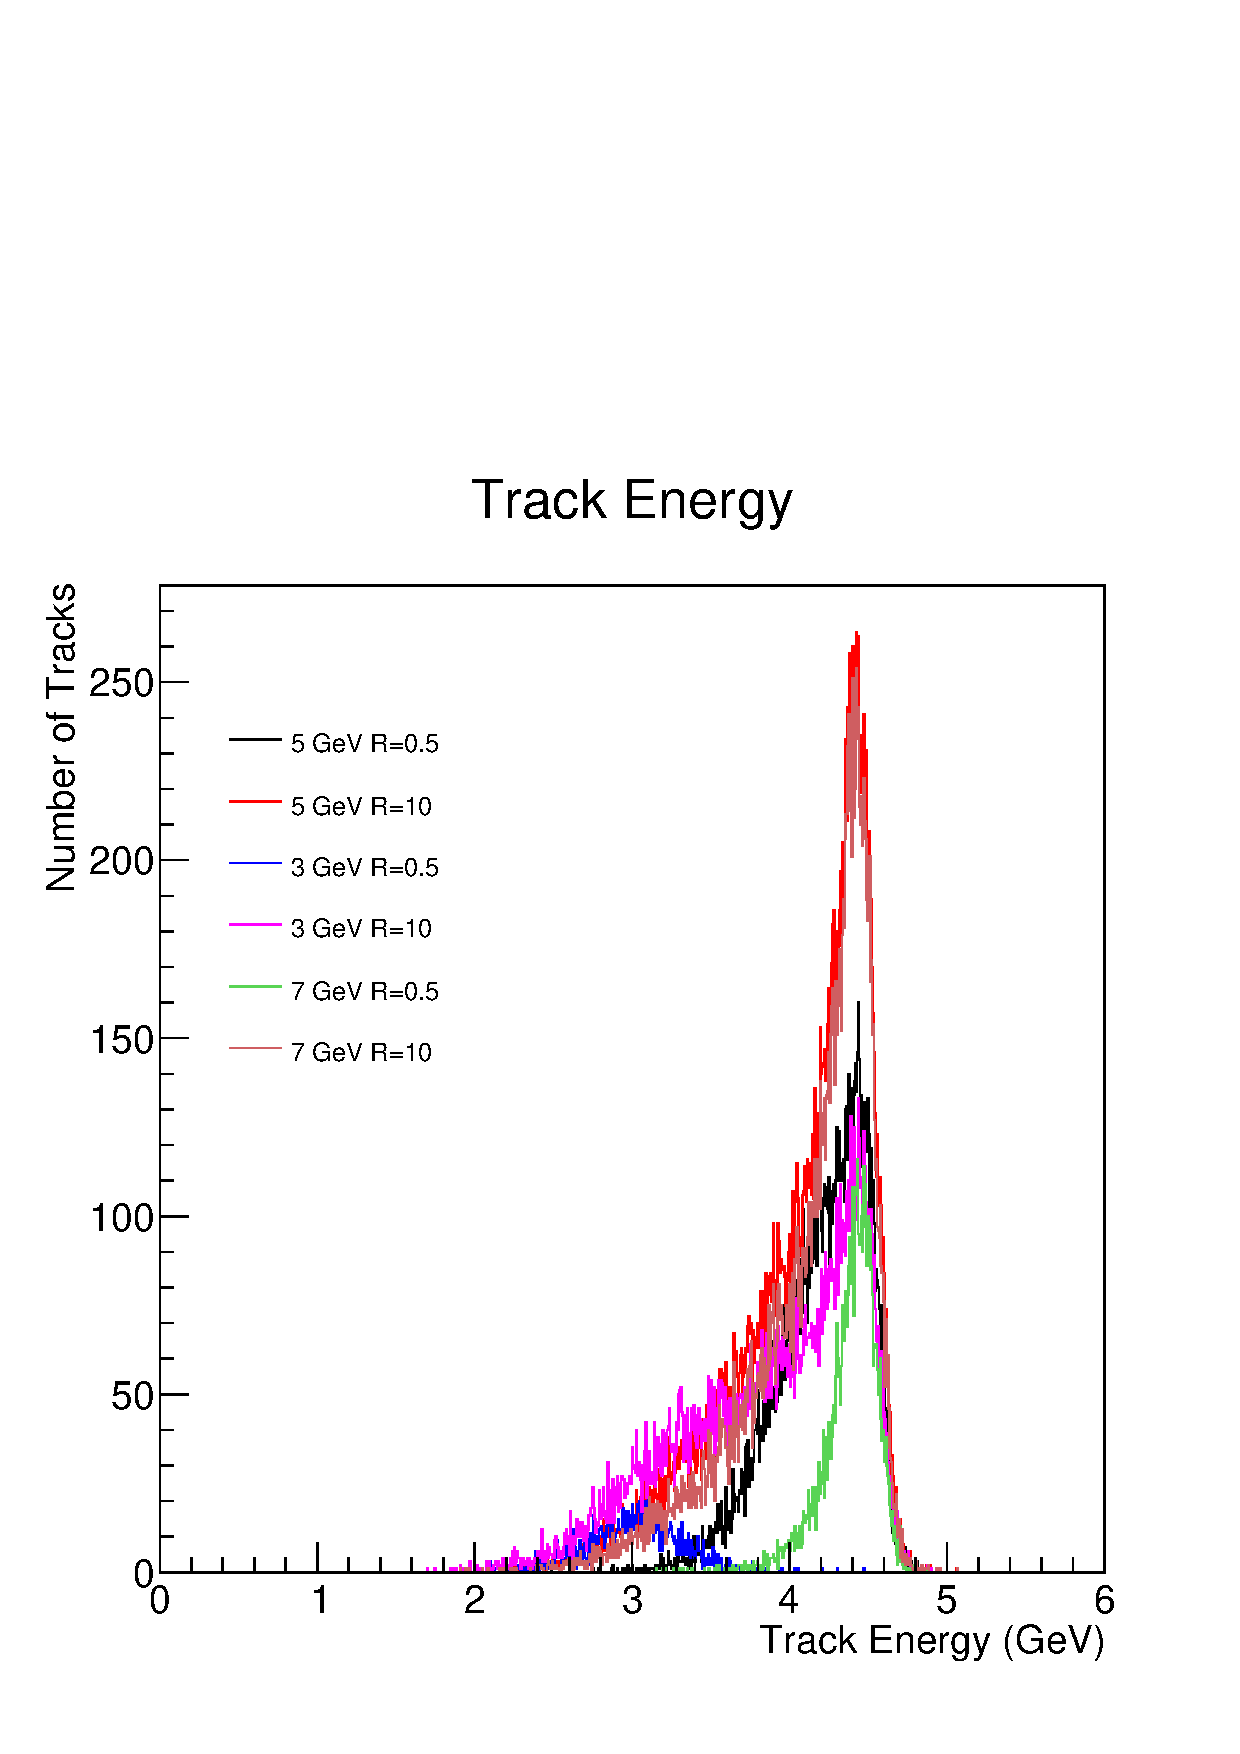
\includegraphics[width=0.65\linewidth]{figures/beamE5B1.pdf}}
\subfloat{\label{fig:chi2E5B1} 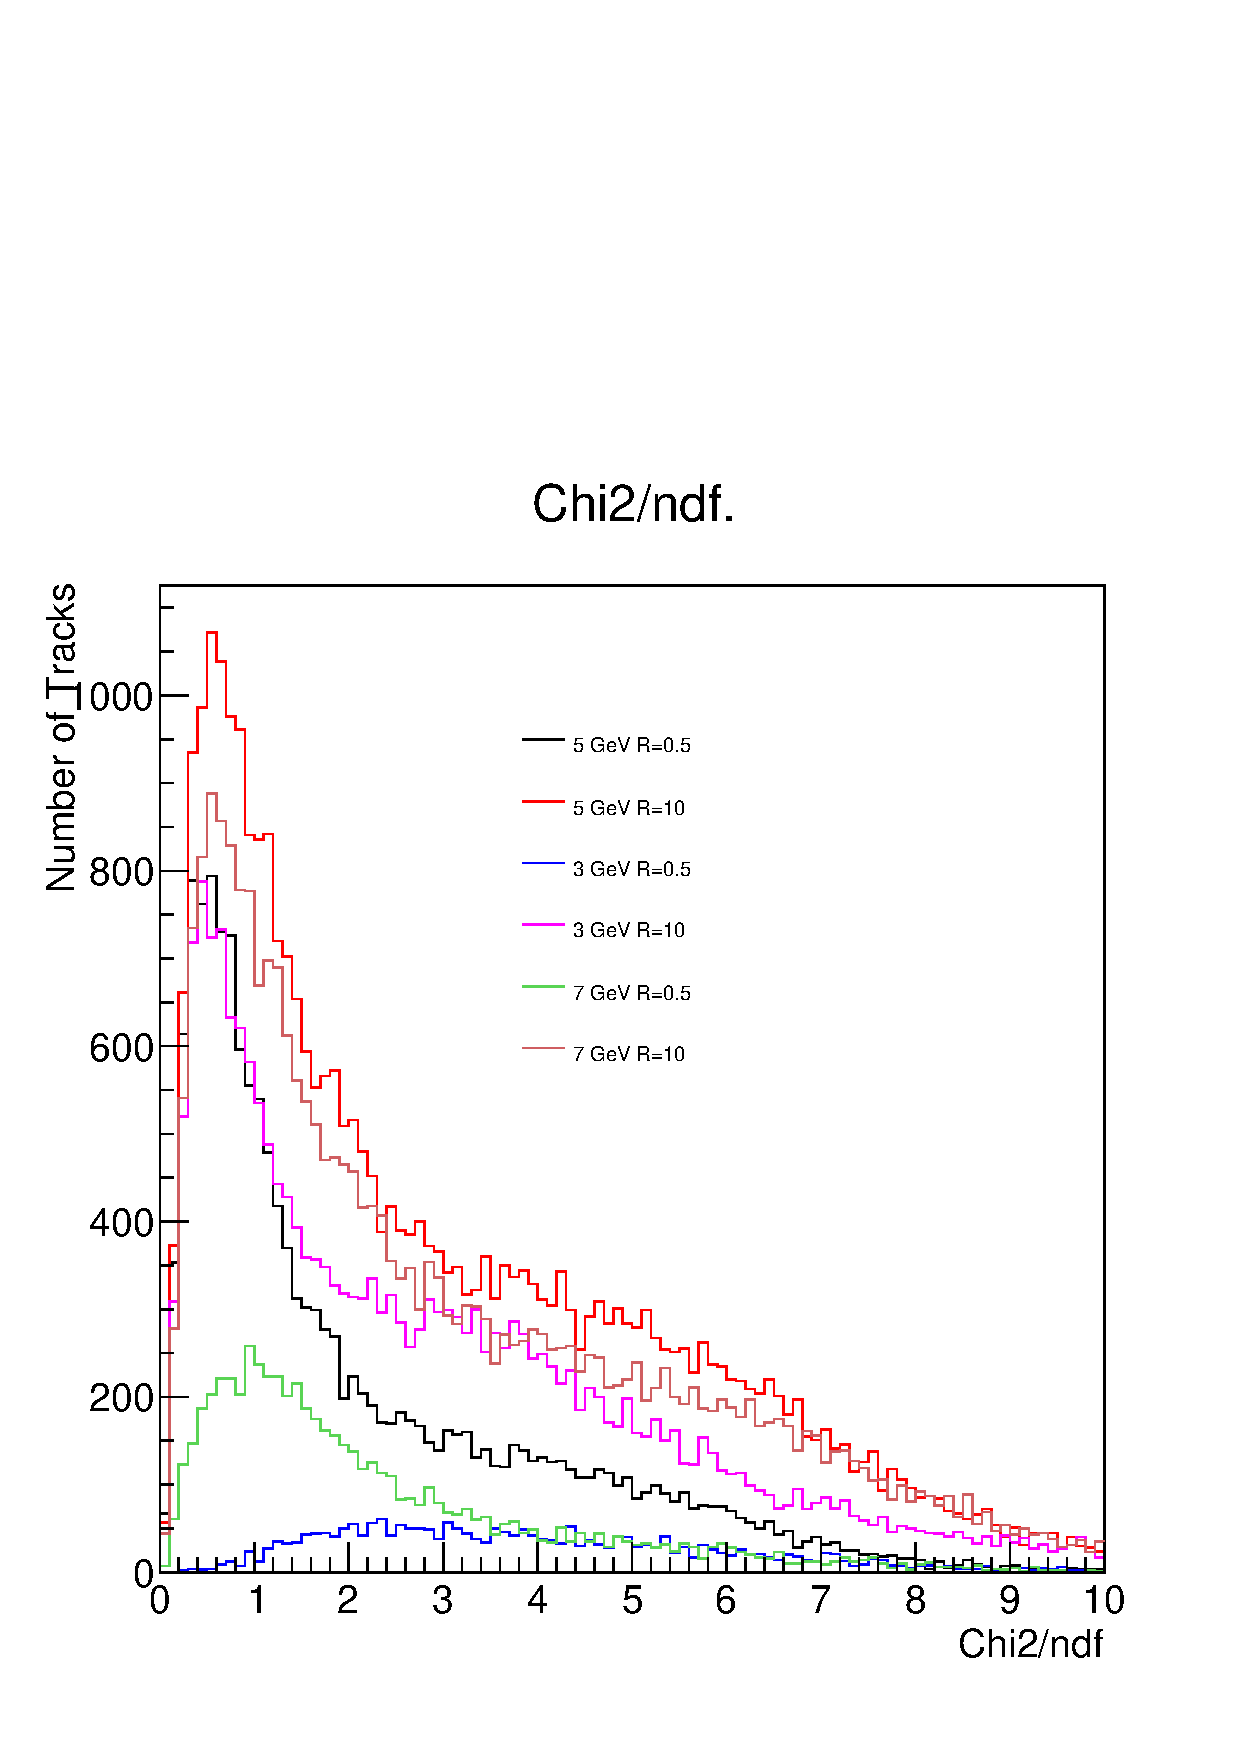
\includegraphics[width=0.65\linewidth]{figures/chi2E5B1.pdf}}
\caption{Figure \ref{fig:beamE5B1} shows the beam energy for a range of pattern recognition inputs, with estimated beam energy 5 GeV and magnetic field 1 T. A cut of  $chi2/ndf > 5$ is made to remove poor tracks for figure \ref{fig:beamE5B1}. Figure \ref{fig:chi2E5B1} shows the chi2 distribution for each fit. }
\label{fig:energy0}
\end{figure}

Note the beam is expected to have some natural spread which is shown. Also observe the drop in energy which is present in both from the expected energy. This is due to the passage of the particle through material which houses the magnet. The pattern recognition has no effect on the mean of the distribution and each is only wider due to larger acceptance of tracks in different regions.  

\begin{figure}[H]
%\centering
\hspace{-2.5cm}
\subfloat{\label{fig:beamE3B1} 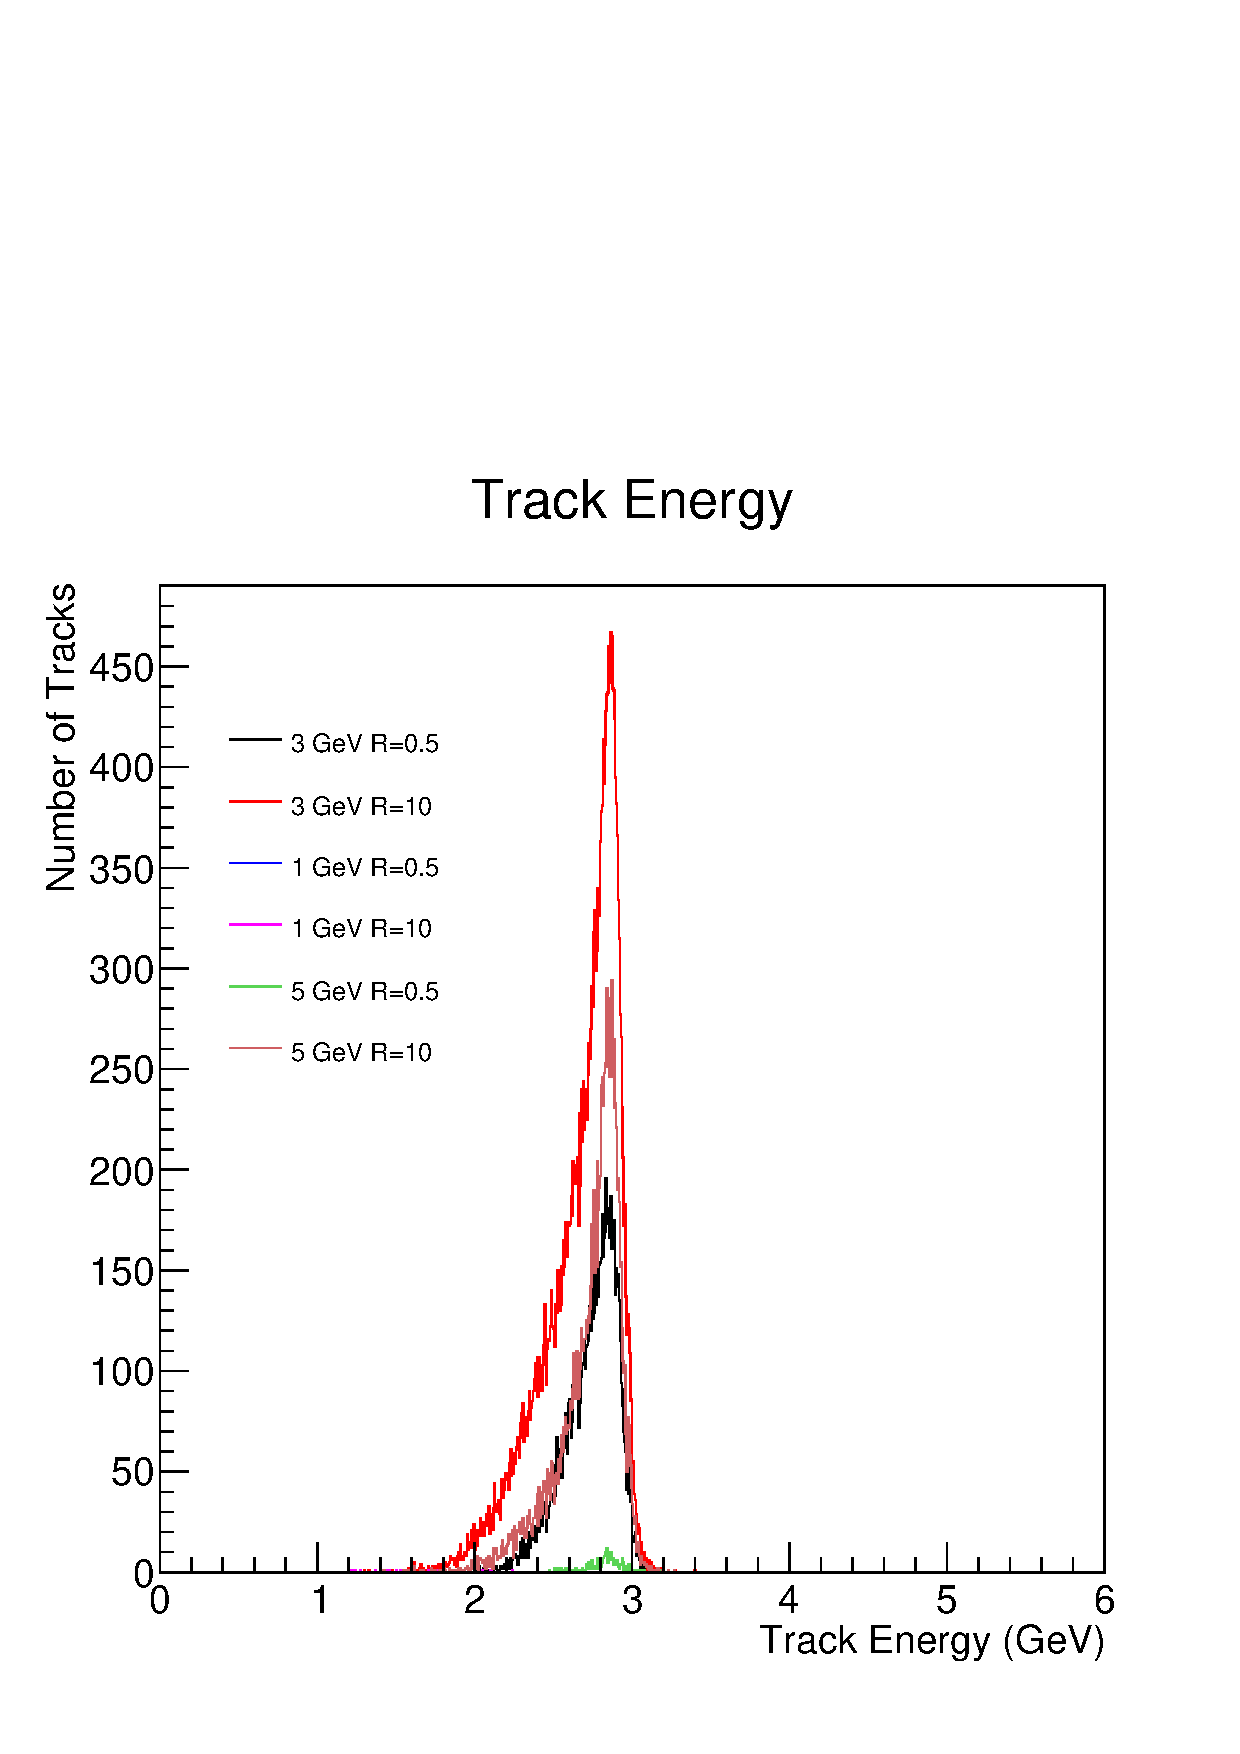
\includegraphics[width=0.65\linewidth]{figures/beamE3B1.pdf}}
\subfloat{\label{fig:chi2E3B1} 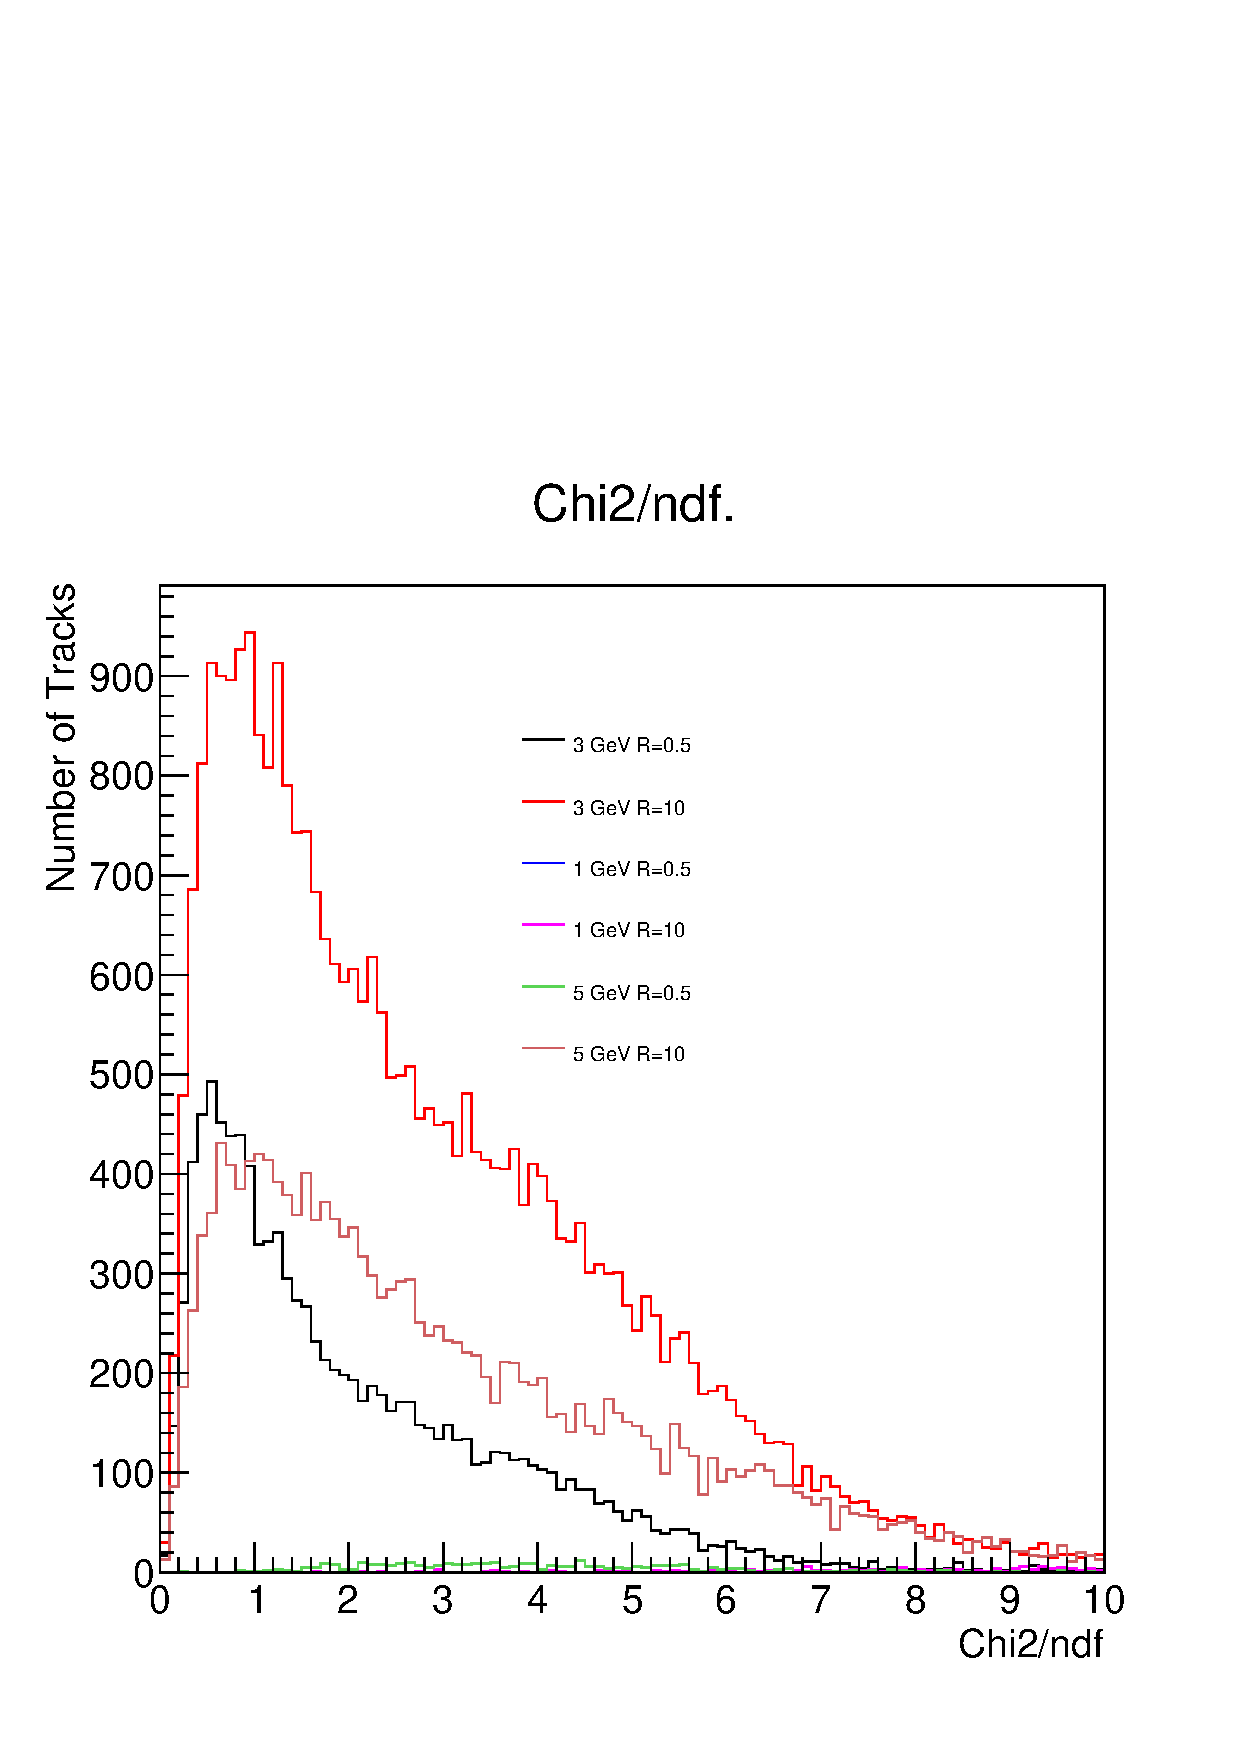
\includegraphics[width=0.65\linewidth]{figures/chi2E3B1.pdf}}
\caption{ Figure \ref{fig:beamE3B1} shows the beam energy for a range of pattern recognition inputs, with estimated beam energy 3 GeV and magnetic field 1 T. A cut of  $chi2/ndf > 5$ is made to remove poor tracks from figure \ref{fig:beamE3B1}. Figure \ref{fig:chi2E3B1} shows the chi2 distribution for each fit.}
\label{fig:energy1}
\end{figure}


